\chapter{Methodik}
\label{chap:Methodik}
\pagestyle{plain}

Im folgenden Abschnitt werde ich die zwei Stücke auf Ihre Phrasierung untersuchen. Dabei starte ich mit der Melodie von \textit{Run To You}, die sich aus den Noten mithilfe von Pausenzeichen in gesungene Phrasen einteilen lässt. Dazu nutze ich die klassische Baumstruktur, die auch \cite{lerdahl1983generative} nutzen und adaptiere diese für die gesungene Phrasierung auf die simpelste Form. Dabei nummeriere ich die Phrasen, um sie später in Kombination mit der Strophen-Nummer eindeutig identifizieren zu können. 

Für eine bessere Übersichtlichkeit, verbinde ich die Phrasen der Melodie nicht miteinander. Auch \cite{hayes1996role} nutzen die Baum-Notation und bedienen sich außerdem der Raster-Notation aus \cite{liberman1975intonational} für die Notation des Rhythmus. Da ich mich in dieser Arbeit nur auf die Untersuchung der Phrasierung beschränke, sind diese Mehr-Informationen jedoch von geringerer Relevanz.



\tiny 

\section*{Run To You}

\subsection*{Melodie}

% HOW? MIT DEN PAUSEN

\subsubsection*{Strophe 1}

\Tree [.Phrase-1 \qroof{A light in the room}. ] 
\Tree [.Phrase-2 \qroof{It was you who was standing there}. ] 
\Tree [.Phrase-3 \qroof{Tried, it was true}. ] 
\Tree [.Phrase-4 \qroof{As your glance met my stare}. ] 
\Tree [.Phrase-5 \qroof{But your heart drifted off}. ] 
\Tree [.Phrase-6 \qroof{Like the land split by sea}. ] 
\Tree [.Phrase-7 \qroof{I tried to go,}. ] 
\Tree [.Phrase-8 \qroof{to follow. To kneel down at your feet}. ] 

\subsubsection*{Refrain 1}

\Tree [.Phrase-1 \qroof{I'll run}. ] 
\Tree [.Phrase-2 \qroof{I'll run}. ] 
\Tree [.Phrase-3 \qroof{I'll run}. ] 
\Tree [.Phrase-4 \qroof{run to you}. ] 
\Tree [.Phrase-5 \qroof{I'll run}. ] 
\Tree [.Phrase-6 \qroof{I'll run}. ] 
\Tree [.Phrase-7 \qroof{I'll run}. ] 
\Tree [.Phrase-8 \qroof{run to you}. ] 

\subsubsection*{Strophe 2}

\Tree [.Phrase-1 \qroof{I've been settling scores}. ] 
\Tree [.Phrase-2 \qroof{I've been fighting so long}. ] 
\Tree [.Phrase-3 \qroof{But I've lost your war}. ] 
\Tree [.Phrase-4 \qroof{And our kingdom is gone. How shall I win back}. ] 
\Tree [.Phrase-5 \qroof{Your heart}. ] 
\Tree [.Phrase-6 \qroof{which was mine}. ] 
\Tree [.Phrase-7 \qroof{I have broken bones}. ] 
\Tree [.Phrase-8 \qroof{and tattered clothes. I've run out of time}. ] 

\subsubsection*{Refrain 2 (siehe oben)}

\subsubsection*{Bridge}

\Tree [.Phrase-1 \qroof{I will break down the gates of heaven}. ] 
\Tree [.Phrase-3 \qroof{A thousand angels stand waiting for me}. ] 
\Tree [.Phrase-3 \qroof{Take my heart and I'll lay down my weapons}. ] 
\Tree [.Phrase-4 \qroof{Break my shackles to set me free}. ] 

\subsubsection*{Refrain 3 (siehe oben)}




\subsection*{Text}

% HOW?

\subsubsection*{Strophe 1}

\Tree [.Phrase-1 \qroof{A light in the room}. ] 
\Tree [.Phrase-2 \qroof{It was you who was standing there}. ] 
\Tree [.Phrase-3 \qroof{Tried, it was true}. ] 
\Tree [.Phrase-4 \qroof{As your glance met my stare}. ] 
\Tree [.Phrase-5 \qroof{But your heart drifted off}. ] 
\Tree [.Phrase-6 \qroof{Like the land split by sea}. ] 
\Tree [.Phrase-7 \qroof{I tried to go,}. ] 
\Tree [.Phrase-8 \qroof{to follow}. ] 
\Tree [.Phrase-9 \qroof{To kneel down at your feet}. ] 

\subsubsection*{Refrain 1}

\Tree [.Phrase-1 \qroof{I'll run}. ] 
\Tree [.Phrase-2 \qroof{I'll run}. ] 
\Tree [.Phrase-3 \qroof{I'll run}. ] 
\Tree [.Phrase-4 \qroof{run to you}. ] 
\Tree [.Phrase-5 \qroof{I'll run}. ] 
\Tree [.Phrase-6 \qroof{I'll run}. ] 
\Tree [.Phrase-7 \qroof{I'll run}. ] 
\Tree [.Phrase-8 \qroof{run to you}. ] 

\subsubsection*{Strophe 2}

\Tree [.Phrase-1 \qroof{I've been settling scores}. ] 
\Tree [.Phrase-2 \qroof{I've been fighting so long}. ] 
\Tree [.Phrase-3 \qroof{But I've lost your war}. ] 
\Tree [.Phrase-4 \qroof{And our kingdom is gone.}. ] 
\Tree [.Phrase-5 \qroof{How shall I win back your heart which was mine}. ] 
\Tree [.Phrase-6 \qroof{I have broken bones and tattered clothes}. ] 
\Tree [.Phrase-7 \qroof{I've run out of time}. ] 

\subsubsection*{Refrain 2 (siehe oben)}

\subsubsection*{Bridge}

\Tree [.Phrase-1 \qroof{I will break down the gates of heaven}. ] 
\Tree [.Phrase-2 \qroof{A thousand angels stand waiting for me}. ] 
\Tree [.Phrase-3 \qroof{Take my heart and I'll lay down my weapons}. ] 
\Tree [.Phrase-4 \qroof{Break my shackles to set me free}. ] 

\subsubsection*{Refrain 3 (siehe oben)}










\section*{Fields Of Gold}

\subsection*{Melodie}

% HOW? MIT DEN PAUSEN

\subsubsection*{Strophe 1}

\Tree [.Phrase-1 \qroof{You’ll remember me when the west wind moves}. ] 
\Tree [.Phrase-2 \qroof{Upon the fields of barley}. ] 
\Tree [.Phrase-3 \qroof{You'll forget the sun in his jealous sky}. ] 
\Tree [.Phrase-4 \qroof{As we walk in fields of gold}. ] 

\subsubsection*{Strophe 2}

\Tree [.Phrase-1 \qroof{So she took her love for to gaze awhile}. ] 
\Tree [.Phrase-2 \qroof{Upon the fields of barley}. ] 
\Tree [.Phrase-3 \qroof{In his arms she fell as her hair came down}. ] 
\Tree [.Phrase-4 \qroof{Among the fields of gold}. ] 

\subsubsection*{Strophe 3}

\Tree [.Phrase-1 \qroof{Will you stay with me? Will you be my love?}. ] 
\Tree [.Phrase-2 \qroof{Among the fields of barley}. ] 
\Tree [.Phrase-3 \qroof{We'll forget the sun in his jealous sky}. ] 
\Tree [.Phrase-4 \qroof{As we lie in fields of gold}. ] 

\subsubsection*{Strophe 4}

\Tree [.Phrase-1 \qroof{See the west wind move like a lover so}. ] 
\Tree [.Phrase-2 \qroof{Among the fields of barley}. ] 
\Tree [.Phrase-3 \qroof{Feel her body rise when you kiss her mouth}. ] 
\Tree [.Phrase-4 \qroof{Among the fields of gold}. ] 

\subsubsection*{Bridge}

\Tree [.Phrase-1 \qroof{I never made promises lightly}. ] 
\Tree [.Phrase-2 \qroof{And there have been some that I've broken}. ] 
\Tree [.Phrase-3 \qroof{But I swear in the days still left}. ] 
\Tree [.Phrase-4 \qroof{We'll walk in fields of gold}. ] 
\Tree [.Phrase-5 \qroof{We'll walk in fields of gold}. ] 

\subsubsection*{Strophe 5}

\Tree [.Phrase-1 \qroof{Many years have passed since those summer days}. ] 
\Tree [.Phrase-2 \qroof{Among the fields of barley}. ] 
\Tree [.Phrase-3 \qroof{See the children run as the sun goes down}. ] 
\Tree [.Phrase-4 \qroof{Among the fields of gold}. ] 

\subsubsection*{Strophe 6}

\Tree [.Phrase-1 \qroof{You’ll remember me when the west wind moves}. ] 
\Tree [.Phrase-2 \qroof{Upon the fields of barley}. ] 
\Tree [.Phrase-3 \qroof{You can tell the sun in his jealous sky}. ] 
\Tree [.Phrase-4 \qroof{When we walked in fields of gold}. ] 
\Tree [.Phrase-5 \qroof{When we walked in fields of gold}. ] 
\Tree [.Phrase-6 \qroof{When we walked in fields of gold}. ] 




\subsection*{Text}

% HOW?

\subsubsection*{Strophe 1}

\Tree [.Phrase-1 \qroof{You’ll remember me}. ] 
\Tree [.Phrase-2 \qroof{when the west wind moves}. ] 
\Tree [.Phrase-3 \qroof{Upon the fields of barley}. ] 
\Tree [.Phrase-4 \qroof{You'll forget the sun}. ] 
\Tree [.Phrase-5 \qroof{in his jealous sky}. ] 
\Tree [.Phrase-6 \qroof{As we walk in fields of gold}. ] 

\subsubsection*{Strophe 2}

\Tree [.Phrase-1 \qroof{So she took her love }. ] 
\Tree [.Phrase-2 \qroof{for to gaze awhile}. ] 
\Tree [.Phrase-3 \qroof{Upon the fields of barley}. ] 
\Tree [.Phrase-4 \qroof{In his arms she fell}. ] 
\Tree [.Phrase-5 \qroof{as her hair came down}. ] 
\Tree [.Phrase-6 \qroof{Among the fields of gold}. ] 

\subsubsection*{Strophe 3}

\Tree [.Phrase-1 \qroof{Will you stay with me?}. ] 
\Tree [.Phrase-2 \qroof{Will you be my love?}. ] 
\Tree [.Phrase-3 \qroof{Among the fields of barley}. ] 
\Tree [.Phrase-4 \qroof{We'll forget the sun}. ] 
\Tree [.Phrase-5 \qroof{in his jealous sky}. ] 
\Tree [.Phrase-6 \qroof{As we lie in fields of gold}. ] 

\subsubsection*{Strophe 4}

\Tree [.Phrase-1 \qroof{See the west wind move}. ] 
\Tree [.Phrase-2 \qroof{like a lover so}. ] 
\Tree [.Phrase-3 \qroof{Among the fields of barley}. ] 
\Tree [.Phrase-4 \qroof{Feel her body rise}. ] 
\Tree [.Phrase-5 \qroof{when you kiss her mouth}. ] 
\Tree [.Phrase-6 \qroof{Among the fields of gold}. ] 

\subsubsection*{Bridge}

\Tree [.Phrase-1 \qroof{I never made promises lightly}. ] 
\Tree [.Phrase-2 \qroof{And there have been some that I've broken}. ] 
\Tree [.Phrase-3 \qroof{But I swear}. ] 
\Tree [.Phrase-4 \qroof{in the days still left}. ] 
\Tree [.Phrase-5 \qroof{We'll walk in fields of gold}. ] 
\Tree [.Phrase-6 \qroof{We'll walk in fields of gold}. ] 

\subsubsection*{Strophe 5}

\Tree [.Phrase-1 \qroof{Many years have passed}. ] 
\Tree [.Phrase-2 \qroof{since those summer days}. ] 
\Tree [.Phrase-3 \qroof{Among the fields of barley}. ] 
\Tree [.Phrase-4 \qroof{See the children run}. ] 
\Tree [.Phrase-5 \qroof{as the sun goes down}. ] 
\Tree [.Phrase-6 \qroof{Among the fields of gold}. ] 

\subsubsection*{Strophe 6}

\Tree [.Phrase-1 \qroof{You’ll remember me}. ] 
\Tree [.Phrase-1 \qroof{when the west wind moves}. ] 
\Tree [.Phrase-2 \qroof{Upon the fields of barley}. ] 
\Tree [.Phrase-3 \qroof{You can tell the sun}. ] 
\Tree [.Phrase-3 \qroof{in his jealous sky}. ] 
\Tree [.Phrase-4 \qroof{When we walked in fields of gold}. ] 
\Tree [.Phrase-5 \qroof{When we walked in fields of gold}. ] 
\Tree [.Phrase-6 \qroof{When we walked in fields of gold}. ] 




\normalsize





\newpage
\subsection*{Run To You}

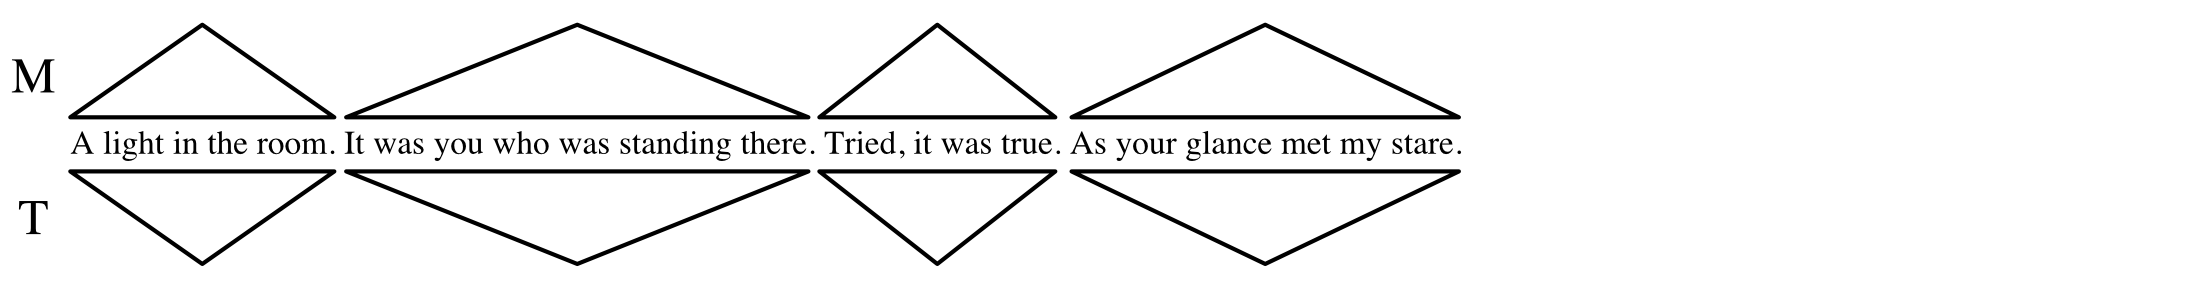
\includegraphics[width=\textwidth]{resources/trees/rty-s1-1.png}
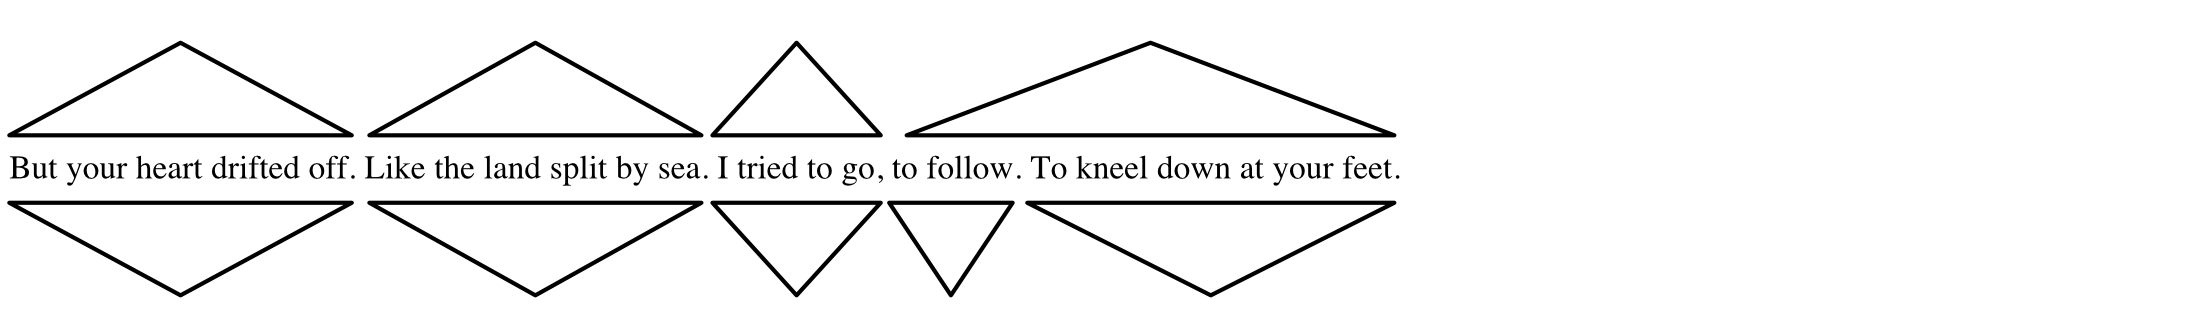
\includegraphics[width=\textwidth]{resources/trees/rty-s1-2.png}
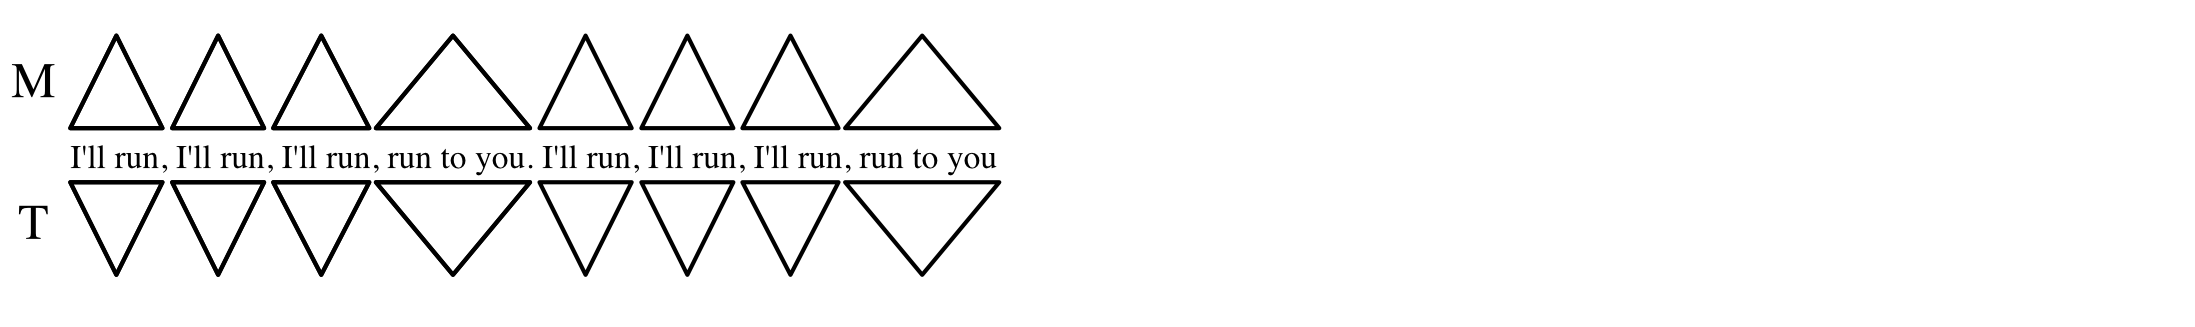
\includegraphics[width=\textwidth]{resources/trees/rty-r.png}
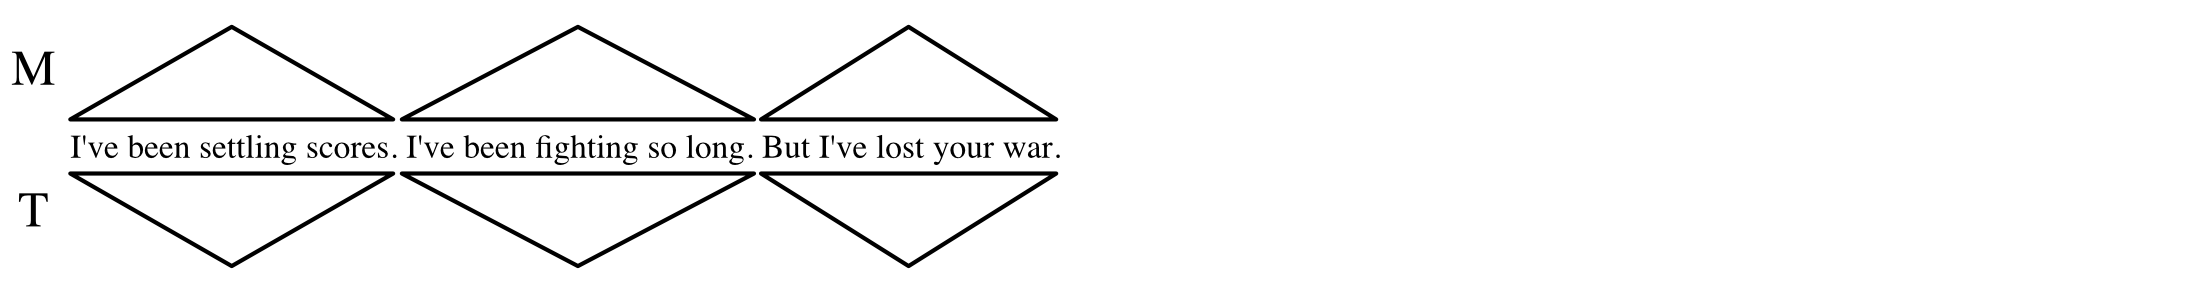
\includegraphics[width=\textwidth]{resources/trees/rty-s2-1.png}
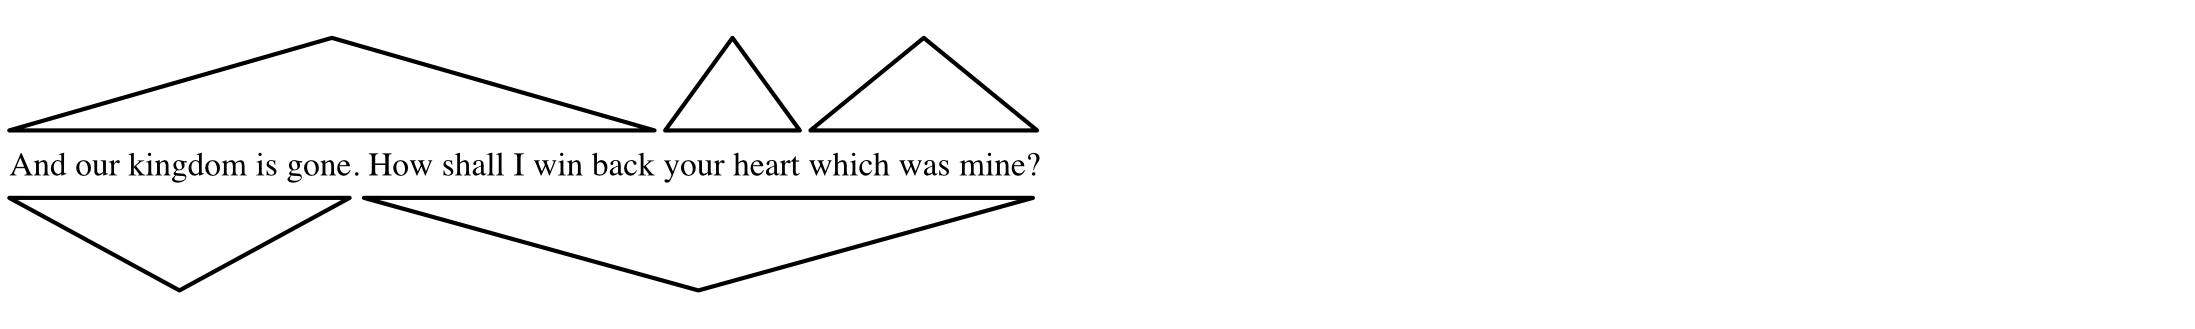
\includegraphics[width=\textwidth]{resources/trees/rty-s2-2.png}
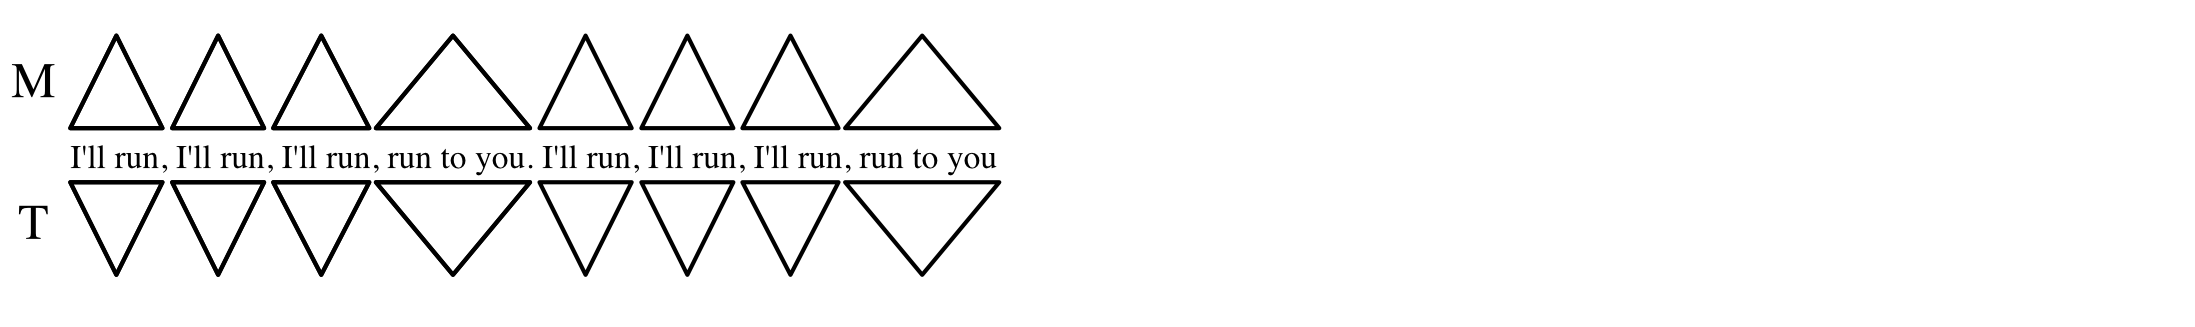
\includegraphics[width=\textwidth]{resources/trees/rty-r.png}
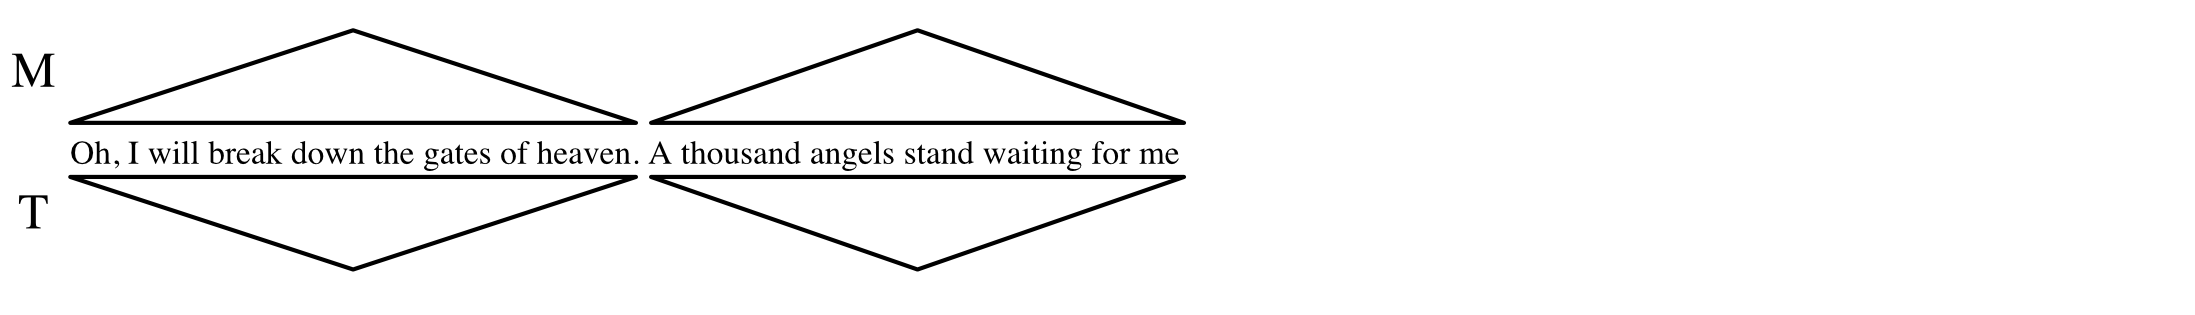
\includegraphics[width=\textwidth]{resources/trees/rty-br-1.png}
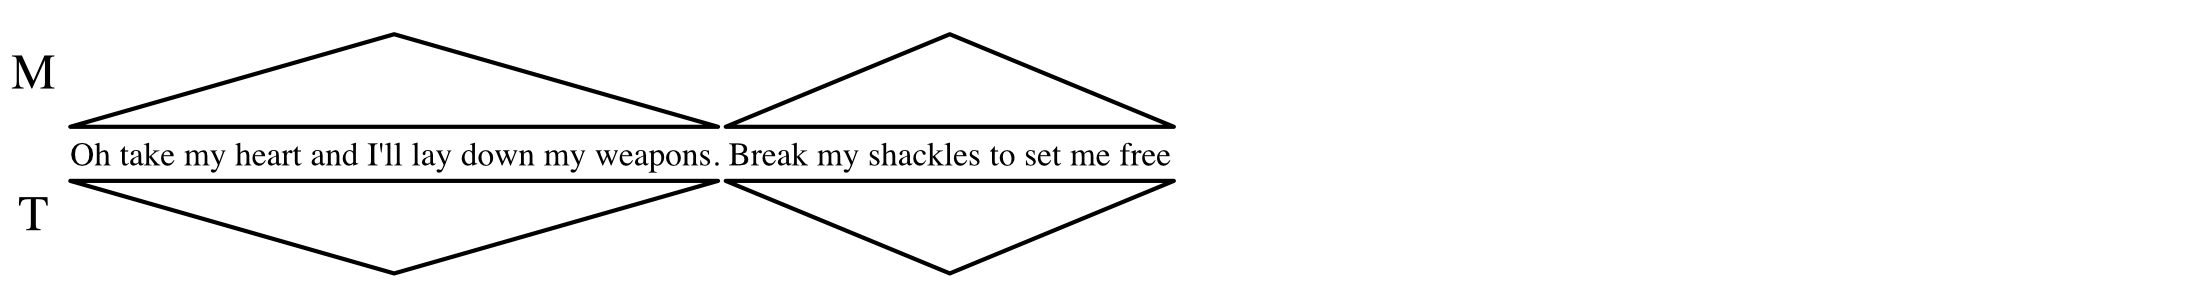
\includegraphics[width=\textwidth]{resources/trees/rty-br-2.png}
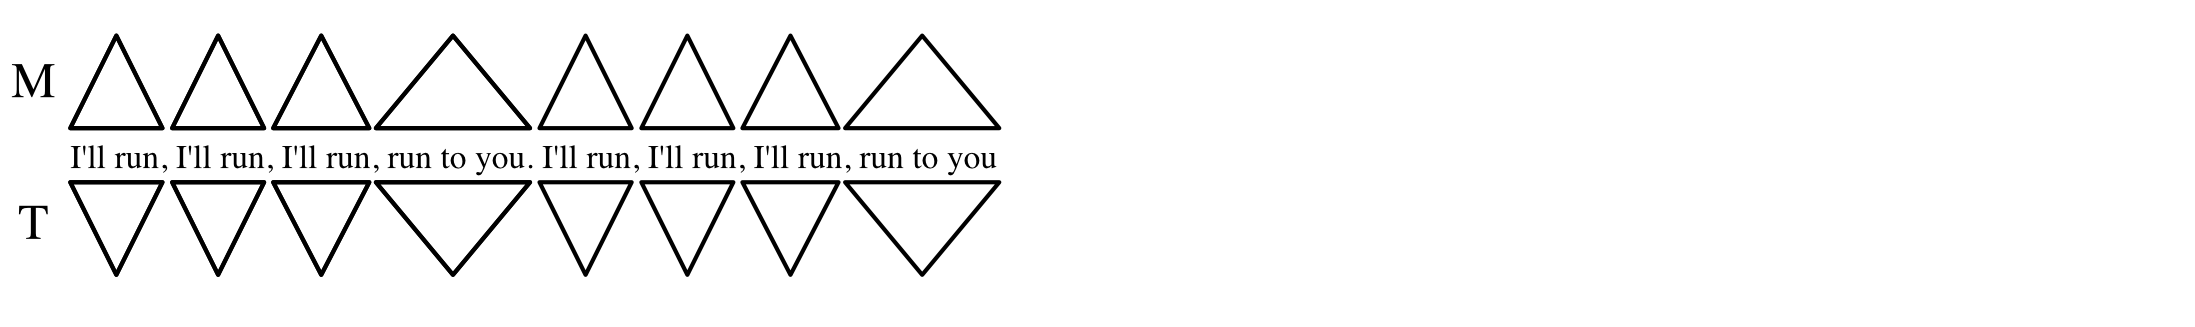
\includegraphics[width=\textwidth]{resources/trees/rty-r.png}

\newpage
\subsection*{Fields Of Gold}

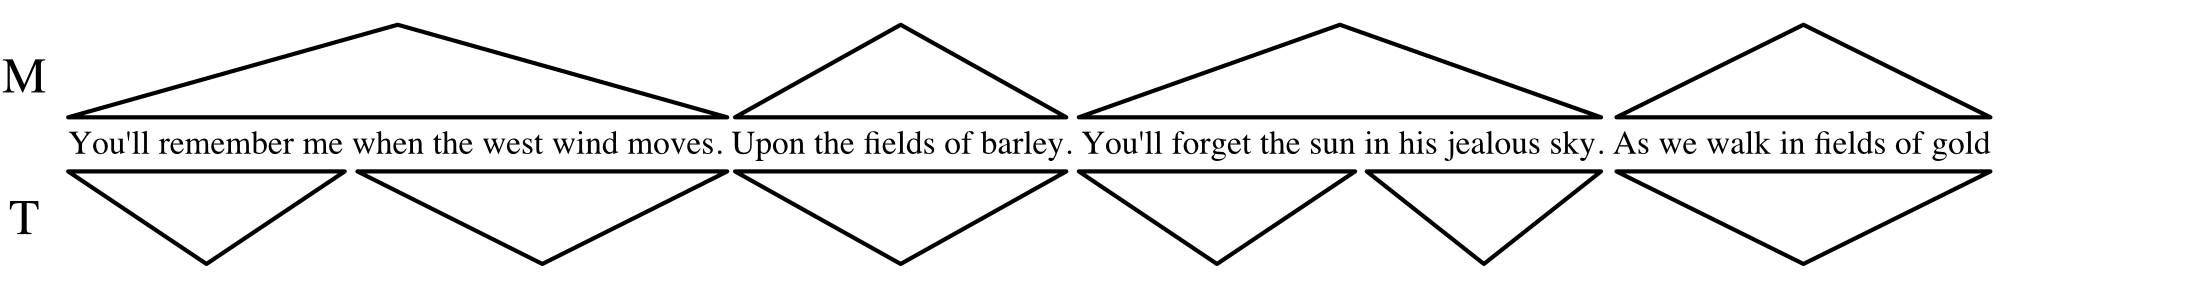
\includegraphics[width=\textwidth]{resources/trees/fog-s1.png}
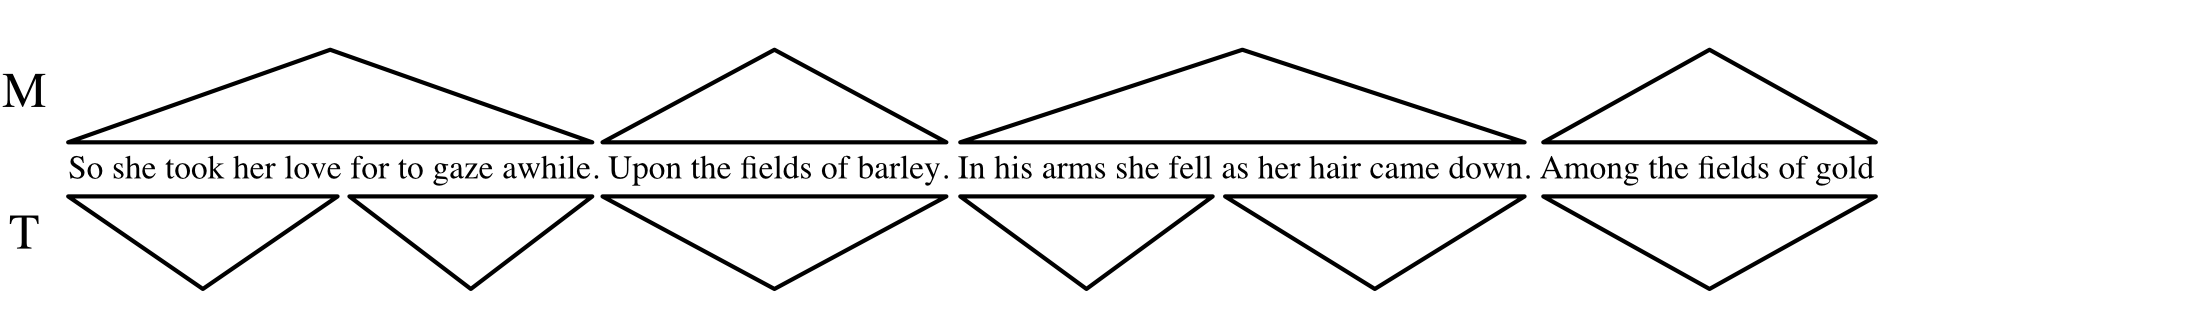
\includegraphics[width=\textwidth]{resources/trees/fog-s2.png}
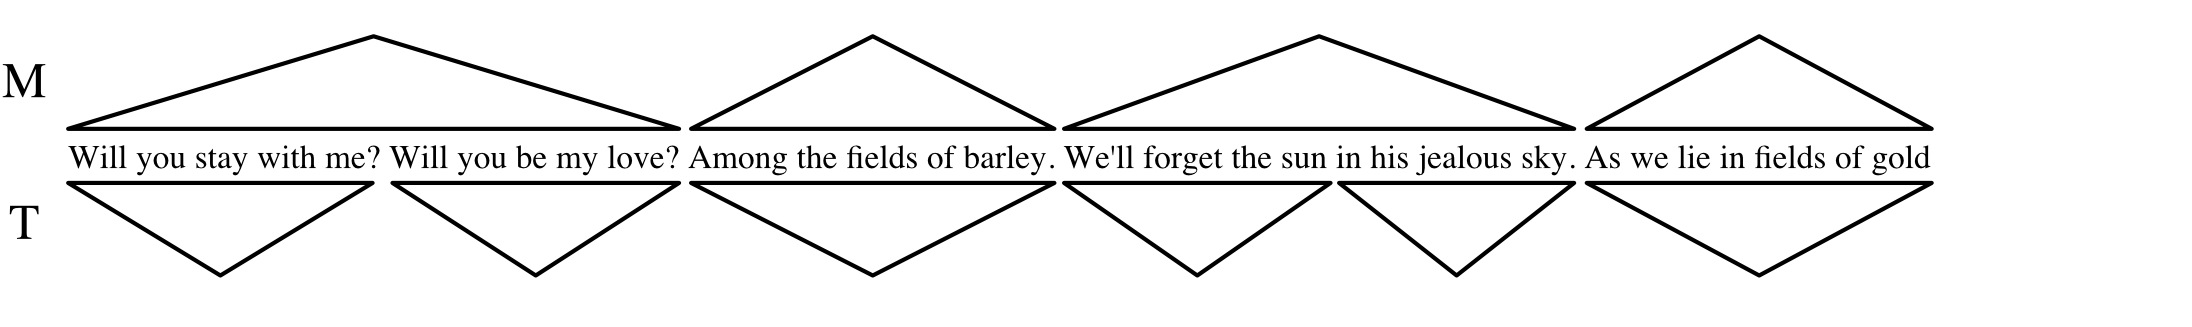
\includegraphics[width=\textwidth]{resources/trees/fog-s3.png}
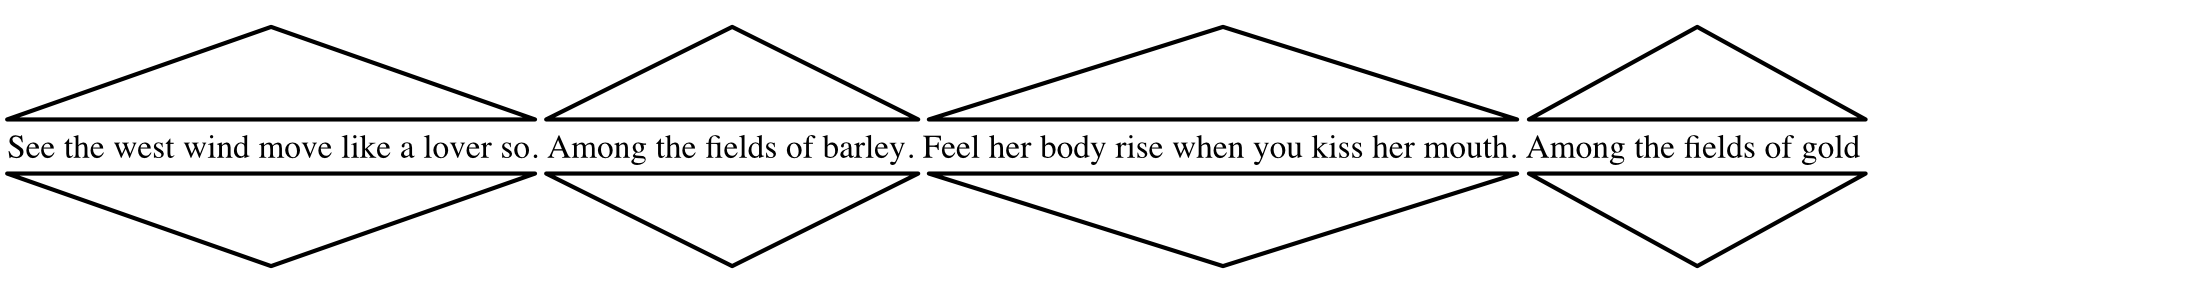
\includegraphics[width=\textwidth]{resources/trees/fog-s4.png}
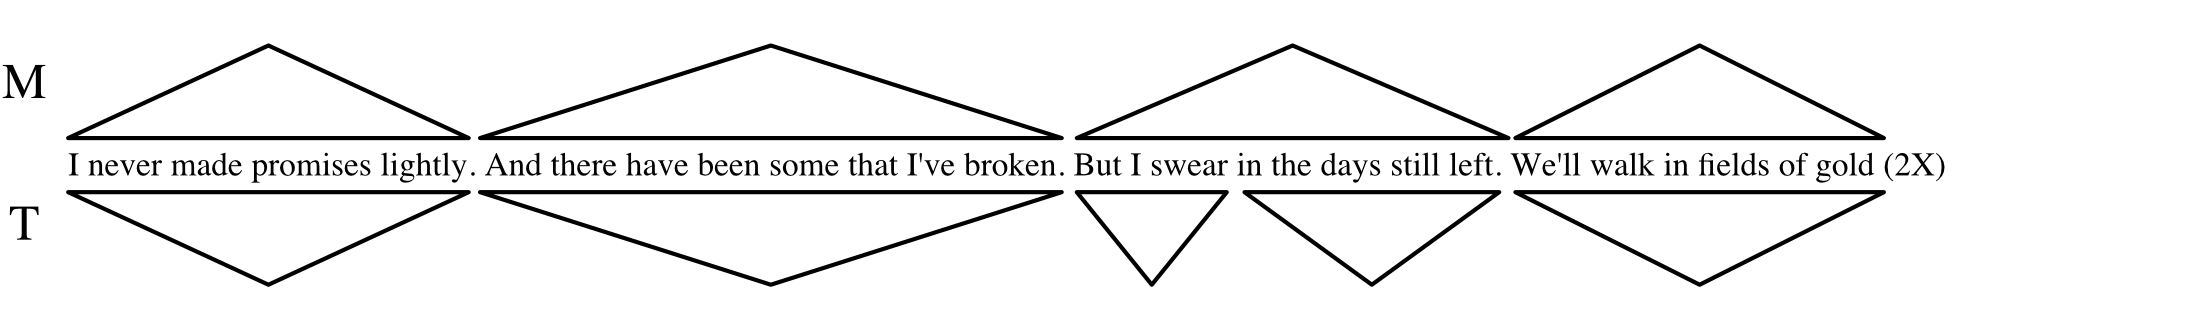
\includegraphics[width=\textwidth]{resources/trees/fog-br.png}
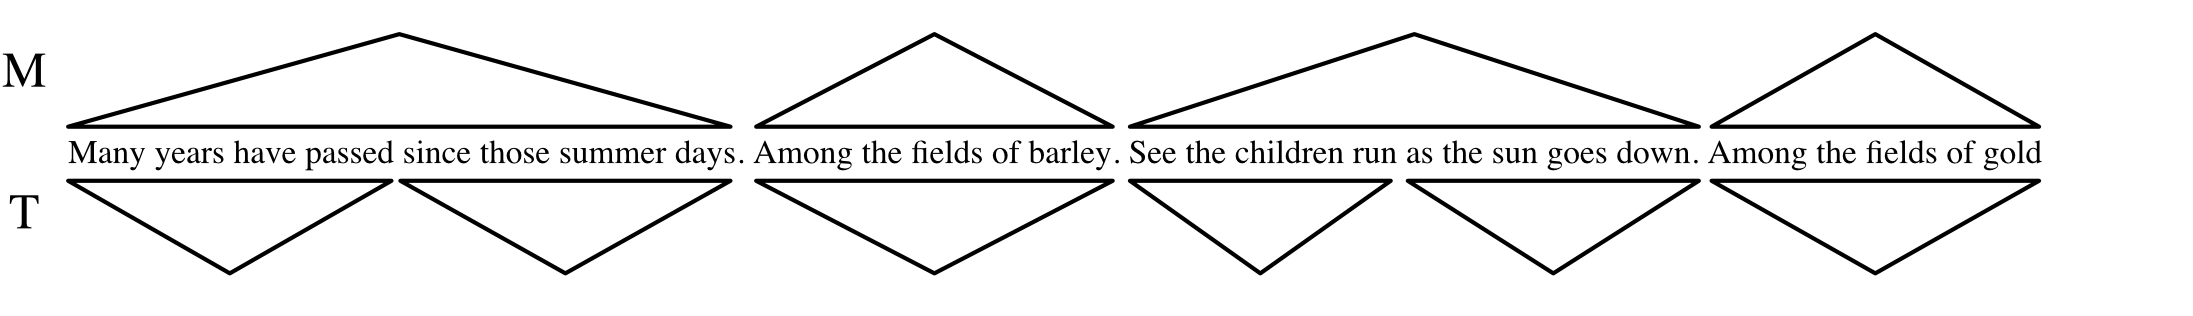
\includegraphics[width=\textwidth]{resources/trees/fog-s5.png}
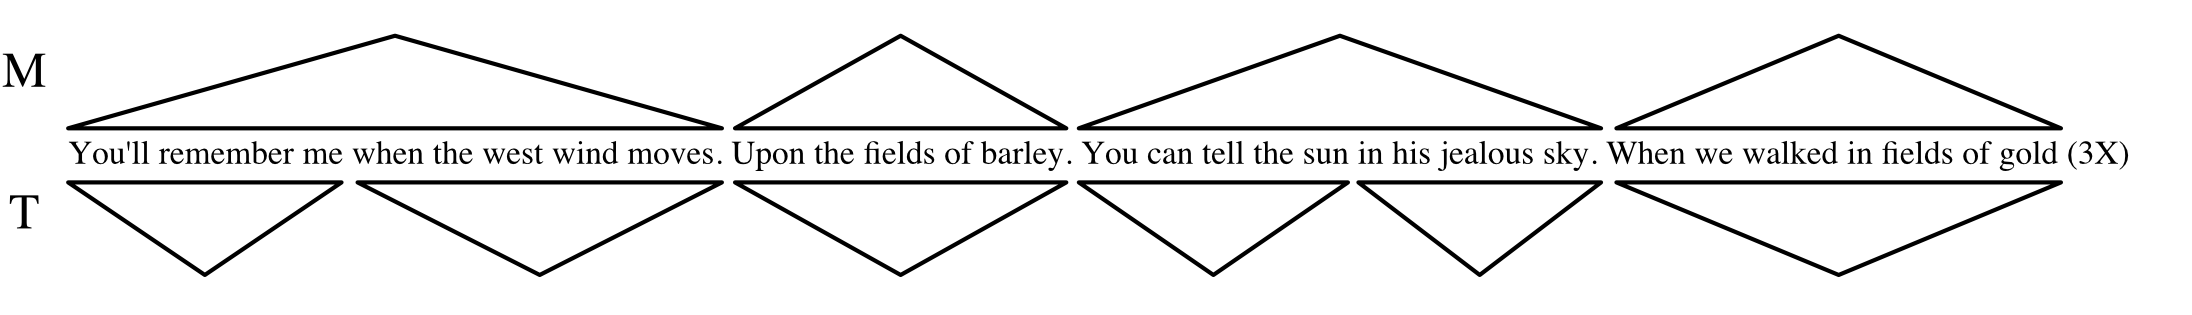
\includegraphics[width=\textwidth]{resources/trees/fog-s6.png}









% quote NLTK as - Bird, Steven, Edward Loper and Ewan Klein (2009), Natural Language Processing with Python. O’Reilly Media Inc.

